\chapter{Previous work} \label{sec:previous_work}

A profusion of techniques 

\section{Food localisation}

%% Color and edge segmentation
%% 11.1

A way to localize food is based on edge detection and colour segmentation.

In \cite{Thendral2014a}, Thendral et al. describes and compare these two methods to localise an orange in a picture. It applied these methods on a small dataset of 20 orange images (only one orange per image), with different lighting conditions and backgrounds (pictures are taken from the Internet).
In more details, the edge-based segmentation apply the canny-edge segmentation, then apply non-maximum suppression to eliminate noises. Then, each pixels are classified.
The colour-based segmentation normalised the lightning condition with a Gaussian low-pass filter, convert the RGB image into a $L * a * b$
\begin{enumerate}
    \item Gaussian low pass filter to normalize the lightning condition
    \item convert the image from RGB representation to $L * a * b$
    \item use the $a$ channel to classify each pixel as \enquote{fruit} or \enquote{non-fruit}
    \item remove small object
    \item fill the binary image regions and holes
\end{enumerate}
For orange detection, the colour segmentation has an higher accuracy. Yet, it is very hard to generalise this method as it has only been tested on oranges, a food item with a very distinctive colour.

%% Circle
%% 2.2 (partial) + 6.3 + \cite{Dehais2015} ?

An other method for food detection relies on circle detection. Indeed, food items are often served in a round shape container such as a bowl, pan or plate.

In \cite{Wazumi2011}, Wazumi et al. describe their use of the Hough transformation. The purpose of this technique is to find approximations of instances a certain class of shapes by a voting procedure. In this paper it is used to detect circles assuming the food is only contained in round plates or bowls and with edges not obstructed on the picture (it performs poorly with cropped pictures). Keeping only the central part of the circle, the segmentation is then fed to the recognition process.

%% CNN
%% DCNN: * ? + 9.1 (in food intake)
%% Presentation of UEC FOOD 100 and 256

A more recent development is the used of convolutional neural network.

In \cite{Shimoda2015}, Shimoda et al. presents their segmentation process based on a pre-trained deep CNN.

The proposed pipeline is composed of 6 main steps:
\begin{enumerate}
    \item detect all the possible bounding box (maximum 2000 per image) using selective search
    \item cluster the bounding box, using the ration of intersection over union (IOU, also call overlap ratio) to obtain 20 at most.
    \item a Deep CNN for all the selected bounding box to get a saliency map. The DCNN is modelled on AlexNet CNN, was pre-trained on the Salient Object Subitizing (14 000 everyday pictures) dataset and fine-tuned on UEC FOOD 100.
    \item use the GrabCut algorithm to extract the foreground region from the food area. GrabCut is an iterative method using graph cuts to extract foreground from background based on an initial guess.
    \item In case of overlapped bounding box, the authors proposed to apply the non-maximum suppression (NMS) algorithm.
\end{enumerate}

The authors apply this process on the UEC-FOOD 100 dataset and PASCAL VOC 2007. The latter is used for object detection and recognition of 20 common classes (train, tv, cat, human ...)). These two datasets use bounding box to spot items. A segmentation is correct if the overlap ratio exceeds 50\% between the predicted and the ground truth bounding box.

UEC FOOD 100 \footnote{Dataset can be found at \url{http://foodcam.mobi/dataset100.html}} is a dataset created by Matsuda et al. in \cite{Matsuda2012a} containing 100 types of food, mainly Japanese food, and is composed of 9060 pictures. Thus, an image can contain multiple dishes. That's why each food picture is associated with the bounding box coordinates indicating the food localisation.

For UEC-FOOD 100, the authors obtain 49.9\% mean average accuracy and 58.7\% for PASCAL VOC 2007.

A pre-trained DCNN is also used by Bolanos et al. \cite{Bolanos2016} to classify each pixel as food or non-food. The DCNN is modelled on \enquote{GoogleNet} \cite{Szegedy2015}, a neural network composed of 22 layers and first used on ILSVRC14 (ImageNet Large Scale Visual Recognition Competition 2014). On UEC-FOOD 256, the authors obtain 60\% of accuracy.

UEC FOOD 256 \footnote{Dataset can be found at \url{http://foodcam.mobi/dataset256.html}} is presented in \cite{Kawano2015} and it is an extension of UEC-FOOD 100 (same creators' team). It adds 156 kinds of food from all the over the world (French, Italian, Vietnamese, American, ...). As for UEC-FOOD 100, every food photo has a bounding box indicating the food location.

\section{Food recognition}

Over the last few years, authors have focused on food recognition. Various methods were tried. For feature extraction, it often combines colour and texture descriptors, global and local.

In \cite{Chen2009}, CHen et al. create a new dataset named PFID and provide two simple food classification baseline methods. PFID (stands for Pittsburgh fast-food image dataset) \footnote{Dataset can be found at \url{http://pfid.rit.albany.edu/}} was presented in \cite{Chen2009} in summer 2008 from the collaboration of Intel Labs Pitssburgh, Columbia and Carnegie Mellon universitie. It is one of the first mature datasets released for food recognition.

It contains 101 meals (categories) from 11 popular fast food chains found in the USA with images and videos captured in both restaurant conditions and controlled lab setting. It contains foods such as chickens, sandwiches, salads, burgers and drinks from Arby's, Bruggers Bagels, Dunkin Donuts, KFC, McDonalds, Panera, Pizza hut, Quiznos, Subway, Taco Bell and Wendy's.

The authors provide :
\begin{itemize}
    \item Colour histogram and SVM classifier. They obtain a mean accuracy of around 12\%.
    \item Bag of SIFT features and SVM classifier. They obtain a mean accuracy of around 25\%.
\end{itemize}

In \cite{Zong2010}, the authors use a local texture feature and their spatial distribution to classify food images from the PFID.

The author use the Bag-Of-Word method; SIFT for detection of the keypoints and LBP for description. The shape context algorithm is used to keep the spatial relationship between codewords (for each image, compute the histogram of one word compared to the others / then mean of the histograms).

For the classification, the authors pick the smallest cost between an image and a food category. For each interest points found with SIFT in the image, we associate a similarity between the point and each visual words of the codebook. The similarity function is based on the Bhattacharyya distance. Then, the shape context between the point of interests and the visual word is calculated and a cost is deduced for each food category. The category with the smallest cost is chosen.

Regrouping the different pictures in 6 main groups the PFI dataset (sandwiches and wraps, meat, salads, donuts, hamburger and miscellaneous), they obtain an average accuracy of 66\%.

Moreover, Fast foods, as they are standardized and have nutrition information available online, can easily be used to measure the calories. In \cite{Wen2009}, the authors are using the PFID's videos to estimate energy intake of a meal.

In \cite{Bosch2011}, the authors use local and global features to identify the food consumed.
For the global features, they use colour properties (entropy, histogram and moments) with texture information provided by Gabor filters. They add local features with the Bag-Of-Features, using SIFT for detection and SIFT, steerable filters and DAISY descriptors. To classify, they use SVM (using the Radial Basis function kernel).
On a in-house dataset (28 classes, 179 images), the authors obtain 86\% of accuracy.

% 4.3 (PFID)

In \cite{Yang2010}, the authors use a novel feature, named PFD (for pairwise local feature distribution) for food recognition and SVM. Then, they apply it on the Pittsburgh fast-food image dataset (PFID) dataset.

The different steps of this method are:
\begin{enumerate}
    \item classify each pixel in one of the categories between beef, chicken, pork, bread, vegetable,  tomato/tomato sauce, cheese/butter, egg/other and background. For classification, they use the Semantic Texton Forest, method based on local characteristics. It was previously trained on 16 manually-labelled pictures.
    
    \item Global ingredient representation (GIR): for the 8 food categories, it sum up the soft label of all the ingredient pixel and normalize by the number.
    
    \item PFD: geometric pairwise feature on N ingredient pixels (picked randomly, thus N / 2 pairs):
    \begin{itemize}
        \item log of the distance
        \item orientation
        \item soft label of the midpoint
        \item soft label of each pixel along the line connecting the pair of pixels
        \item joint feature (a mixed of the above characteristics)
    \end{itemize}
    Accumulate the pairwise values into a distribution (using a multi-dimensional histogram of either 8 or 12 bins), weighted by the soft labels of the two pixels. Each pixel is mapped to its closest bin in the histogram.
    Then, normalization of the histogram.
\end{enumerate}

For the PFID dataset, they obtain an accuracy between 19\% and 28\% for each of the 61 categories.
When they pick the 6 major types of food, they get almost 80\% of accuracy.

% ETHZ Food 101
% 2.1

In \cite{Bossard2014}, the author use the Random forest clustering algorithm to create superpixels (selecting only the discriminative one). On these superpixels, a dense SURF and L*a*b* color value is computed and encoded with improved fisher vectors (IFV) with Gaussian mixture model (GMM) of 64 Gaussians.
Then, they use PCA to reduce the size of the vector and the machine learning method is structured-output multi-class SVM. They use their method on their new dataset named ETHZ Food-101 (56\% accuracy) and MIT-indoor (58\% of accuracy on the full dataset) and compare it against several previous implementations.

ETHZ Food-101 \footnote{Dataset can be found at  \url{https://www.vision.ee.ethz.ch/datasets_extra/food-101/}} is composed of 101 categories, 1000 images per category (250 pictures manually reviewed, used for the test set and 750 with noises for the training test). Pictures were extracted from the website \href{http://www.foodspotting.com/}{foodspotting.com}. The top 101 most popular dishes from this social sharing food images defined the categories.

% 8.3

\cite{Chen2012} present a method to automatically identify food and estimate the quantity. It is used on an in-house dataset composed of 50 categories, mainly Chinese fishes, with 100 pictures per class. For recognition, the authors use:
\begin{itemize}
    \item local information with Bag-Of-Words, using SIFT as descriptor and Local binary pattern on a 3-level pyramid
    \item global information: colour histograms and Gabor filters extracted from of each block (image divided into $4 \times 4$ blocks)
\end{itemize}

They train a SVM classifier for each category, then fuse them with the multi-class AdaBoost algorithm. AdaBoost, or \enquote{Adaptive boosting} is a meta-algorithm that combine into a weighted sum multiple classifiers to improve their final performance.
The authors get an overall accuracy of 68.3\%. If we keep the top-3 results, the accuracy is even 90.9\%.


%% DCNN

More recently, people have started to heavily use Convolutional Neural Networks \textit{CNN} with great results.

%% UMPC Food 101
%% 8.1

In \cite{Wang2015}, the authors created a new dataset named UMPC Food-101 ("twin dataset" of ETHZ Food 101) combining text and visual information for recipes. As a proof of concept, they develop a search application for recipe recognition. The user send a query (a food image) and as a result, the three best recipes (categories) are displayed.

UMPC Food-101 \footnote{Dataset can be found at \url{http://visiir.lip6.fr/}} is a \enquote{twin-dataset} of ETHZ Food 101 as it is composed of the same 101 categories, with 1000 images per category. Yet, the pictures have been crawled from Google image, researching for recipes. Thus, most images are associated with a text.

For the image recognition model, they use textual, visual or a mix of both features:
\begin{itemize}
    \item visual feature (all feeding a SVM):
    \begin{itemize}
        \item Bag-of-Words using a dense SIFT and a codebook of size 1024 on a 3-level spatial pyramid. They obtain an average accuracy of 23.96\%.
        
        \item Use an improved version of the Bag-of-Words named \enquote{BossaNova}. It modifies the pooling system; instead of keeping the closest cluster of a SIFT descriptor, it represents it by keeping distances between the descriptor and all the codebook words. Average accuracy of 28.59\%.
        
        \item Use a deep CNN as a feature descriptor, using the 7th layer of a pre-trained CNN ("OverFeat"). Average accuracy of 33.91\%.
        
        \item Use a very deep CNN as a feature descriptor, using th 19th layers ("vgg-verydeep-19"). Average accuracy of 40.21\%.
    \end{itemize}
    
    \item text-feature: use the term frequency - inverse document frequency \textit{tf-idf} method and get 82.06\% accuracy
    
    \item fusion of textual and visual feature: they obtain at most 85.10\% of accuracy, combining the very deep CNN descriptors and tf-idf.
\end{itemize}

%% UEC FOOD
%% 2.3

In \cite{Kawano2014}, the authors use a pre-trained Deep CNN \textit{DCNN} for feature extraction. The DCNN, called \enquote{OverFeat}, \footnote{Can be found \url{http://cilvr.nyu.edu/doku.php?id=code:start}} was trained on ImageNet and is composed of 19 layers. The authors add more conventional image features to obtain feature vectors composed of: 
\begin{enumerate}
    \item a variant of the Histogram of Oriented Gradients \textit{HOG} called \enquote{Root Hog} that is an element-wise square root of the L1 normalized HOG
    \item mean and variance values of each channel of the RGB representation value of pixels from each of 2*2  block
    \item the last two layers of the DCNN
\end{enumerate}
The three descriptors are then encoded in a fisher vector. Using SVM, the authors obtain 72\% of  accuracy for UEC-FOOD 100.

%% UEC FOOD 256

In \cite{Yanai2015}, the authors use a fine-tuned pre-trained DCNN with the large-scale ImageNet dataset for food recognition. The authors obtain 79\% average accuracy for UEC FOOD 100 and 67\% for UEC FOOD-256.

In \cite{Bolanos2016}, the authors also use a fine-tuned pre-trained Deep Neural Network and obtain 63\% accuracy on UEC FOOD-256. Their neural network is fine-tuned on multiple food datasets (UEC FOOD 256, Food 101 and EgocentricFood).

\section{Food intake estimation}

%% Food Log

FoodLog \footnote{\url{http://www.foodlog.jp}} is a website that enables the user to upload pictures of its daily meals to be archived and processed. The goal of this application is to assist the user to keep notes of their meals and balance the nutritional values coming from different kinds of food.

In \cite{Kitamura2008}, the images containing food items are identified by exploiting features related to the HSV and RGB colour domains, as well as the shape of the plate. A SVM classifier is trained to detect food images. More specifically, the images are divided in 300 blocks and each block is classified as \enquote{non-food} (discarded block) or one of the nutritional categories described in the \enquote{MyPyramid} model \footnote{\url{http://www.mypyramid.gov}}.

MyPyramid \cite{MyPyramid} was designed by the United State Department of Agriculture \textit{USDA} in 2005 and was replaced in 2011 by \enquote{MyPlate} \footnote{\url{http://www.choosemyplate.gov}} \cite{MyPlate}. This dietary model is composed of 5 kinds of food: grains, vegetable, meals and beans, milk and fruit. For each group, a recommended intake per day is associated, Fig. \ref{fig:my_pyramid}. Quantity is categorized by \enquote{servings} \textit{SV}, making it simpler to compute and keep log.

\begin{figure}
    \centering
    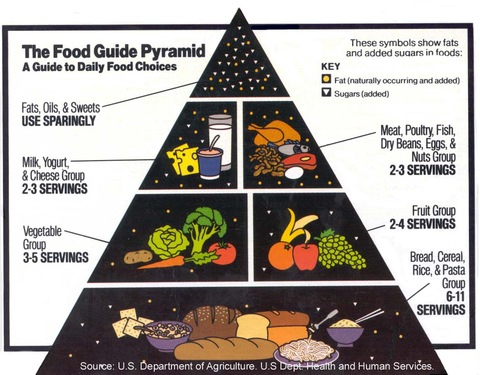
\includegraphics[scale=0.7]{img/my_pyramid.jpg}
    \caption[USDA MyPyramid original logo]{USDA MyPyramid original logo. Source \href{https://en.wikipedia.org/wiki/Food_pyramid_(nutrition)}{Wikipedia}.}
    \label{fig:my_pyramid}
\end{figure}

In \cite{Aizawa2013} the Support Vector Machine is replaced by a Bayesian Framework \textit{BF}.
The BF is based on the Gaussian Naive Bayesian (suppose independence between every pair of features and the distribution of each feature is assumed to be Gaussian). The BF takes into account the estimation using colour moments and Bag-Of-Feature of SIFT, the prior distribution and the mealtime category (breakfast, lunch and dinner).

In \cite{Kagaya2014}, the authors use a Convolutional Neural Network \textins{CNN} to detect and classify food from a small subset of image loaded in the FoodLog system. Compared to the other conventional methods (use of a feature descriptor such as Bag-of-Words with a classifier, e.g. SVM) described previously, the CNN showed a significantly higher accuracy.

%% Others

An other method to estimate the food intake is to evaluate the food volume.

In \cite{Chen2012}, the authors presents a method that use the depth information of the picture. Once the food has been classified, the area of the food container (bowl, plate) and the depth value of the contained food is computed to obtain the food volume.
Yet, this technique is still limited as it can only be used for non-transparent food, i.e it can't detect some food item such as water or cooked rice, and force the user to have a depth camera (such as Kinect).

In \cite{Almaghrabi2012a}, the authors presents a novel food recognition system that is able to estimate of the nutrition intake. Moreover, they develop a mobile application to easily take pictures and keep track of the user's diet.
To measure the food intake, authors compare before and after eating pictures and use the thumb as the calibration system (it supposes a one-time calibration to know the size of the thumb of the user).
The process to show the intake is:
\begin{enumerate}
    \item the user takes food pictures
    \item get the contour of each picture
    \item recognition of the food using colour, shape and size features with SVM.
    \item volume calculation, that is computed in two steps:
    \begin{enumerate}
        \item user takes a picture from above. Then, the food shape is divided into known shape (rectangle, circle, triangle ...) to compute the area.
        \item user takes a second picture from the side. This is used to compute the height of the food and calculate the overall volume.
    \end{enumerate}
    The system assumes that the plate is white and round.
    \item use a nutrition database to obtain the average calories
\end{enumerate}
If the user has not eaten everything, the entire must be repeated.
The drawbacks of this method is the user have to take several pictures, with one's thumb each time and it has been tested with a limited set of simple food types.

%
% Zhu
%

In \cite{Zhu2010}, the authors develop a mobile application to keep food records of a user that is taking pictures of one's meal. Their method can detect multiple food items in one picture. They use a colour marker (color chequerboard) as an illumination and size indicator.
As in \cite{Almaghrabi2012a}, images obtained before and after foods are eaten are used to estimate the amount of food consumed.

When the user upload a picture, it is segmented, then classified by a back-end server. The estimation (labelled image with food type and volume) are sent back to the user for confirmation.

For segmentation, the authors use connected component analysis, active contours, and normalized cuts. Then, colour and texture features are extracted to feed a SVM classifier. The authors use:
\begin{itemize}
    \item Gabor filters. Gabor filters describe properties related to the local power spectrum of a signal and have been used for texture analysis
    \item 2-D colour histograms of the a* and b* channels of the CIELaB representation. Values are corrected using the colour marker
\end{itemize}
For the volume estimation, the authors use a 3-D volume reconstruction process. The food area is partitioned and assigned to \enquote{geometric classes}, each with their own sets of parameters.

They evaluate their segmentation and classification methods on a very small dataset composed of 63 images and 19 classes. The authors obtain an average accuracy of 89\%.

In \cite{Zhu2015}, their method is named \enquote{multiple hypotheses segmentation and classification} \textit{MHSC}. It is an iterative algorithm composed of a segmentation, description (extraction of features) and classification steps.

For segmentation, the authors first detect salient region, using Canny edge and colour distribution to reject background. Then, they apply a multi-scale segmentation using normalized cut. Small segmented regions are discarded.

On the selected region, the authors used a mixed of global descriptors (first and second moment of each channel for RGB, YCbCr, L*a*b*, and HSV colour spaces, first and second moment of the entropy in RGB, predominant colour descriptor, entropy and two first moments of the Gradient Orientation Spatial-Dependence Matrix, entropy categorization and fractal dimension estimation and estimation of the fractal dimension of the response of different Gabor filter) with local feature (multi Bag-Of-Words using SIFT for RGB, SURF for RGB, SIFT for each channel of the RGB representation and steerable filters).

Each of the 12 descriptor, global and local, is classified independently and assigned a confidence score. A late fusion function (either maximum confidence score or majority vote) is used  to decide the final class. For classification, the authors use K-NN and SVM.

If the total score is inferior to a certain threshold, the overall process is repeated. The confidence score of the previous step is used to improve the segmentation.

Applied on a dataset composed of 83 labels (79 food classes plus \enquote{utensils}, \enquote{glasses}, \enquote{plates}, and \enquote{plastic cups} classes), each class having at least 30 images, they obtain a top-8 accuracy of 75\%, using K-NN with the maximum confidence score.

%% Food Cam
%% 6.3

In \cite{Matsuda2012a}, the authors propose a food recognition system named \textbf{FoodCam} to identify food items of a picture. The presented process is used on a mobile application, the user taking a picture that is transferred to a sever, processed and results are displayed.

The first step is to detect potential region with multiple object detection algorithms. Then, for these regions, several feeatures are extracted and used to feed SVM with Multiple Kernel Learning \textit{MKL} method. To detect candidate regions, the authors use:
\begin{itemize}
    \item Felzenszwalb’s deformable part model (DPM), based on Histogram of Oriented Gradients (HOG).
    \item a circle detector: the image is converted to a gray-scale, contour are extracted using the Canny Edge Detector and circles detected by the Hough Transform
    \item JSEG region segmentation: segment region based on colour. It only keeps circular regions.
    \item whole image, for picture with one large dish
\end{itemize}
Then, it aggregates all the candidate regions to get the bounding box of each food item.

For each region, it extracts multiple common features:
\begin{itemize}
    \item Bag of Feature of SIFT and C-SIFT (sift with colour invariant characteristics)
    \item Spatial pyramid representation: object regions are divided by hierarchical grids. In this paper, the three level pyramid is used: $1 \times 1$, $2 \times 2$, $3 \times 3$. For each grid, a BoF vector is extracted
    \item Histogram of Oriented Gradient (HOG)
    \item Gabor texture
\end{itemize}

After extraction of the feature vectors from each candidate region, a linear SVM trained by MKL is used ($\chi^2$ kernel). Their methods were evaluated on UEC-FOOD 100. For multiple food item images, they obtain 55.8\% classification rate and 68.9\% for single food item pictures.

%% 

In \cite{Kawano2014a}, the authors develop a mobile real-time food recognition system for calorie and nutrition estimation. Contrary to the previous paper, all the calculation are realised on the user smartphone. The recognition takes less than 1 second thanks to the multi-core architecture of modern smartphones.
The user takes a picture and draws bounding boxes around food items. Then, the system refine the segmentation based on the users' rough demarcation using Grabcut.
For each item, it extracts image features and classify the image among the one hundred food classes using a linear SVM. Then, the top five food candidates are shown and the user can select one of the proposition.
This recognition is updated every one second, the direction arrow as presented in Fig. \ref{fig:food_cam} being displayed to help the user improve the result by changing the camera position and direction. To estimate the most suitable direction, the authors use the Efficient Sub-window Search method, a recent and powerful window search algorithm used in object detection.
The mobile application keep records of all the pictures and their approved classification and labelled with the volume estimation. Food intake is estimated thanks to a slider on the bottom-left of the screen.

\begin{figure}
    \centering
    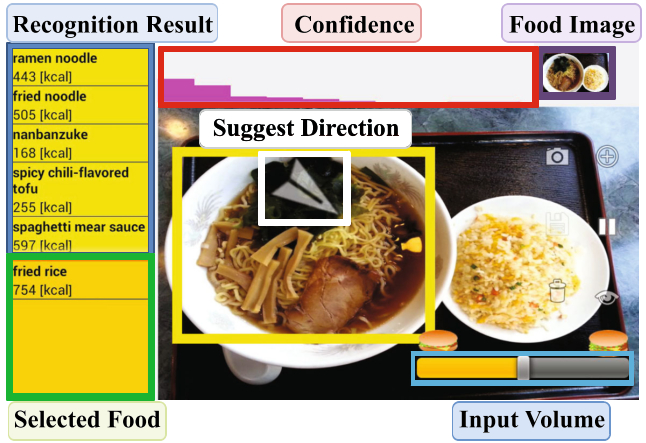
\includegraphics[scale=0.6]{img/foodcam.jpg}
    \caption[Annotated screenshot of the FoodCam application]{Annotated screenshot of the FoodCam application. Source \cite{Kawano2014a}.}
    \label{fig:food_cam}
\end{figure}

Two different descriptors are used:
\begin{itemize}
    \item bag-of-feature, SURF for detection and description, and colour histogram with the $chi^2$ kernel feature map
    \item HOG and a colour patch descriptor (mean and variance of RGB values on a $2 \times 2$ blocks of pixel) encoded using Fisher Victor, a patch encoding strategy using Gaussian mixture models.
\end{itemize}
The authors evaluate these two methods on UEC-FOOD 100. Taking the top 5 classes, they obtain 79\% classification accuracy for colour patches and 68\% for the other.

%% 11.2

In \cite{Bettadapura2015}, the authors develop an application to recognize food items from an image taken by the user in a restaurant. It uses some contextual data (the geolocalisation) to improve the classification. Indeed, they use geolocalisation to get the menu from internet and query Google Search to get images (extract the top 50 pictures) of 15 dishes from the menu. These images are used as weakly-labelled training pictures to improve the recognition accuracy.

The first step is the segmentation to localize the food and ignore the background through hierarchical segmentation. Then, colour moment invariants, hue histograms, Bag of Words of SIFT, RGB SIFT (SIFT component for each RGB channel), C-SIFT (a color invariant SIFT), Opponent-SIFT (SIFT on colour-opponent channels) are used as feature descriptors. For the 4 SIFT representations: they build a codebooks of 100 000 visual words (using k-means clustering, k = 1000) to build Bag-of-Word histogram.

Then, for the image classification, they adopt the SMO-MKL (Sequential minimal optimization - Multiple kernel learning) multi-class SVM (preceded by $\chi^2$ kernel) methods.

It is applied on these two datasets:
\begin{itemize}
    \item PFID to compare to existing recognition systems. Their method obtain 48.5\% accuracy.
    
    \item in-house dataset consisting of images from 10 restaurants (divided in 5 different types of food: American, Indian, Italian, Mexican and Thai). It is made up of 600 pictures, 300 taken with a smartphone, 300 with Google glasses. The overall average accuracy is 63.33\%, only 15.67\% without localization.
\end{itemize}